
\documentclass[a4paper,12pt]{article}
\usepackage[a4paper,top=1.3cm,bottom=2cm,left=1.5cm,right=1.5cm,marginparwidth=0.75cm]{geometry}
\usepackage{cmap}					
\usepackage[warn]{mathtext} 		
\usepackage[T2A]{fontenc}			
\usepackage[utf8]{inputenc}			 
\usepackage[english,russian]{babel}	
\usepackage{longtable}
\usepackage{float}
\restylefloat{table}
\usepackage{graphicx}
\usepackage{tabularx}
\usepackage{hyperref}
\usepackage[rgb]{xcolor}
\usepackage{amsmath,amsfonts,amssymb,amsthm,mathtools} 
\mathtoolsset{showonlyrefs=true}
\usepackage{euscript}
\usepackage{mathrsfs}
\date{\today}
\begin{document}

\begin{titlepage}
	\begin{center}
		{\large МФТИ}
	\end{center}
	\begin{center}
		{\large ФРКТ}
	\end{center}
	
	
	\vspace{4.5cm}
	{\huge
		\begin{center}
			{\bf Лабораторная работа 5.2.1}\\
			Опыт Франка-Герца.
		  
		

		\end{center}
	}
	\vspace{9cm}
	\begin{flushright}
		{\LARGE  $\newline$Добровольская Ксеня$\newline$Гаврилин Илья$\newline$
			\vspace{0.2cm}
			Б01-110$\newline$}
	\end{flushright}
	\vspace{8cm}
	
\end{titlepage}

\section{Аннотация}


  В данной работе предлагалось измерить значения энергии возбуждения первого уровня атома гелия и сравнить результаты с табличным значением $E = 21.6$ эВ. Для этого мы провели опыт Франка и Герца в двух следующих режимах:
  $\newline$ 
1.) Динамическом. Значение этой величины cocтавило  $E_1 = (15.3 \pm 0.6) eB$, что отличается от табличного значения на 29 \%.

2.) Статическом. Значение этой величины составило $E_1 = (21.5 \pm 0.6) eB$, что отличается от табличного значения всего лишь на 0.5\% и совпадает с учетом погрешности.
  $\newline$
  $\newline$
  
\section{Опыт Франка и Герца}
  
      \begin{figure}[H]
  \begin{center}
    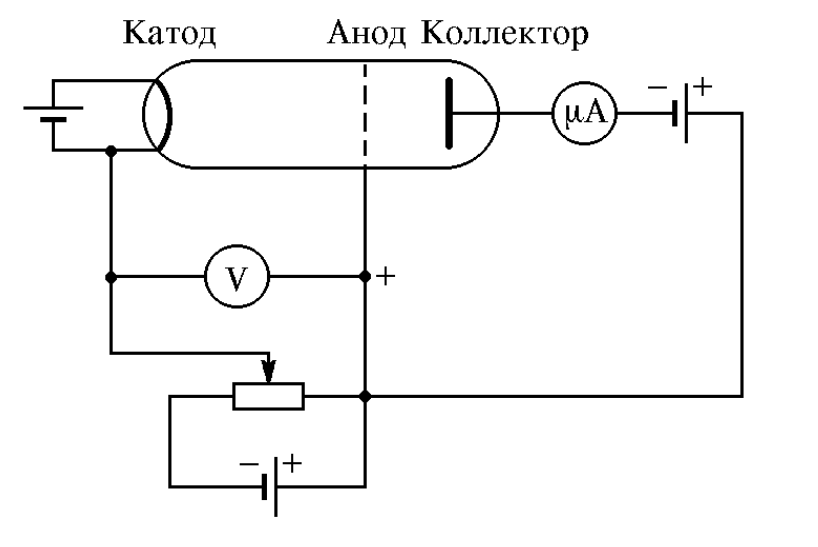
\includegraphics[width=10cm]{ex1.png}
    \caption{Принципиальная схема опыта Франка и Герца.}
    \label{fig:}
  \end{center}
\end{figure}
 
 
 Одним из простых опытов, подтверждающих существование дискретных уровней энергии атомов, является эксперимент, известный под названием опыта Франка и Герца. Схема опыта изображена на рис. 1.
	$\newline$$\newline$
	Разреженный одноатомный газ (в нашем случае — гелий) заполняет трехэлектродную лампу. Электроны, испускаемые разогретым катодом, ускоряются в постоянном электрическом поле, созданном между катодом и сетчатым анодом лампы и сталкиваются с атомами гелия. Если энергия электрона, налетающего на атом, недостаточна для того, чтобы перевести его в возбужденное состояние, то возможны только упругие соударения.
	$\newline$$\newline$
	По мере увеличения разности потенциалов между анодом и катодом энергия электронов увеличивается и, в конце концов, оказывается достаточной для возбуждения атомов. При таких -- неупругих -- столкновениях кинетическая энергия налетающего электрона передается одному из атомных электронов, вызывая его переход на свободный энергетический уровень (возбуждение) или совсем отрывая его от атома (ионизация).
	$\newline$$\newline$
	Ток коллектора, пропорциональный числу электронов, попадающих на него за секунду, измеряется микроамперметром.
$\newline$$\newline$
	При увеличении потенциала анода ток в лампе вначале растет. Однако, когда энергия электронов становится достаточной для возбуждения атомов, ток коллектора резко уменьшается. При дальнейшем увеличении потенциала анода ток коллектора вновь возрастает.
$\newline$$\newline$
	Следующее замедление роста тока происходит в момент, когда часть
	электронов неупруго сталкивается с атомами два раза: первый раз посередине пути, второй -- у анода и т. д. Таким образом, на кривой зависимости тока коллектора от напряжения анода имеется ряд максимумов и минимумов, отстоящих друг от друга на равные расстояния $\Delta V$. Эти расстояния равны энергии первого возбужденного состояния.
	
	
\section{Экспериментальная установка} 
   
   
Схема экспериментальной установки приведена на рис.2.
  
    \begin{figure}[H]
  \begin{center}
    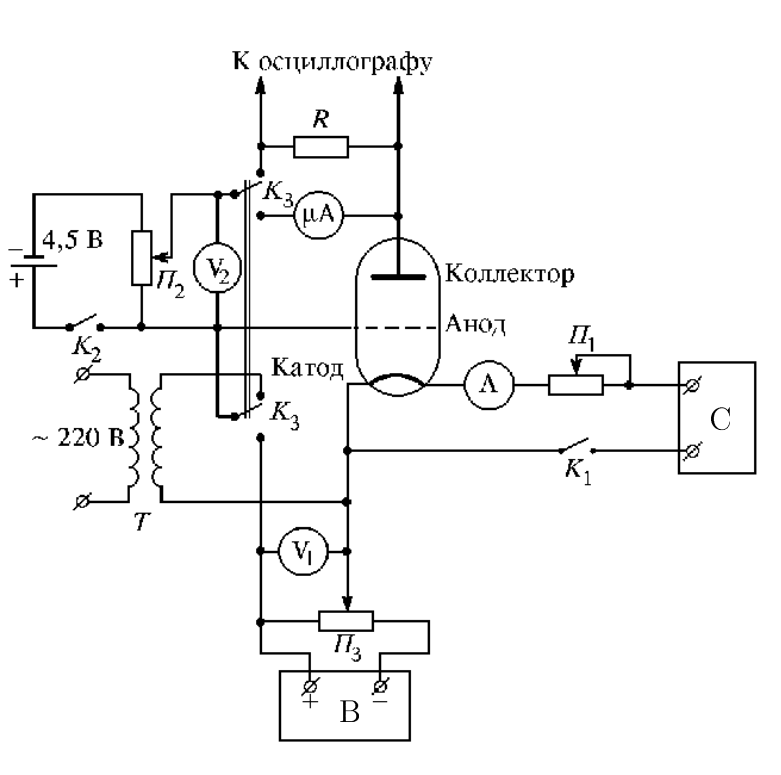
\includegraphics[width=10cm]{ex2.png}
    \caption{Схема экспериментальной установки.}
    \label{fig:}
  \end{center}
\end{figure}
 
 Схема экспериментальной установки изображена на рис. 2. Для опыта используется серийная лампа ионизационного манометра ЛМ-2, заполненная гелием. Напряжение накала подается от стабилизированного источника питания Б7-4. Ток накала контролируется амперметром А. Источник Б7-4 включается в цепь тумблером К$_1$.
	$\newline$$\newline$
	В качестве анода используется двойная спираль, окружающая катод. Роль коллектора играет полый металлический цилиндр, соосный с катодом и анодом.
	$\newline$$\newline$
	Ускоряющее напряжение подается на анод от выпрямителя Б5-10. Величина этого напряжения регулируется потенциометром П$_3$ и измеряется вольтметром $V_1$. Источник задерживающего потенциала -- батарея КБСЛ (4,5 В) -- включается ключом K$_2$, величина потенциала регулируется потенциометром П$_2$ и измеряется вольтметром $V_2$. Ток в цепи коллектора регистрируется микроамперметром.
$\newline$$\newline$
	Схему можно переключать из статического режима измерений в динамический режим с помощью ключа K$_3$. На рис.2 две части сдвоенного ключа K$_3$ изображены отдельно. При динамическом режиме работы ускоряющий потенциал подается с понижающего трансформатора $T$ (220/50 В), а ток коллектора регистрируется осциллографом, подключенным к нагрузочному резистору $R$. Осциллограф следует синхронизировать от сети 50 Гц.
$\newline$$\newline$
	При определении энергии электронов по разности потенциалов между анодом и катодом следует иметь в виду, что из-за контактной разности потенциалов между катодом и анодом первый максимум не соответствует потенциалу первого возбужденного уровня. Однако контактная разность потенциалов так сдвигает все максимумы, что расстояние между ними не меняется.
 

\section{Динамический режим} 
 
 
 \begin{enumerate}
\item При максимальном ускоряющем напряжении измеряем на экране осциллографа расстояния по оси x между первым и вторым максимумами $\Delta{V_1}$ и между вторым и третьим $\Delta{V_2}$ для трех значений задерживающего напряжения V:
  
\textbf{Чувствительность канала X} — 1 В/дел.

\textbf{Чувствительность канала Y} — 1 мВ/дел.

  \begin{table}[H]
\begin{center}
\begin{tabular}{|c|c|c|c|}
\hline $V $, B&$\Delta{V_1}$, дел &$\Delta{V_2}$, дел& $\Delta{V_{cr}}$, дел\\
\hline 4&15&17&16\\
\hline 6&14&16&15\\
\hline 8&14&16&15\\
\hline 
\end{tabular}
\end{center}
\end{table}

    \begin{figure}[H]
  \begin{center}
    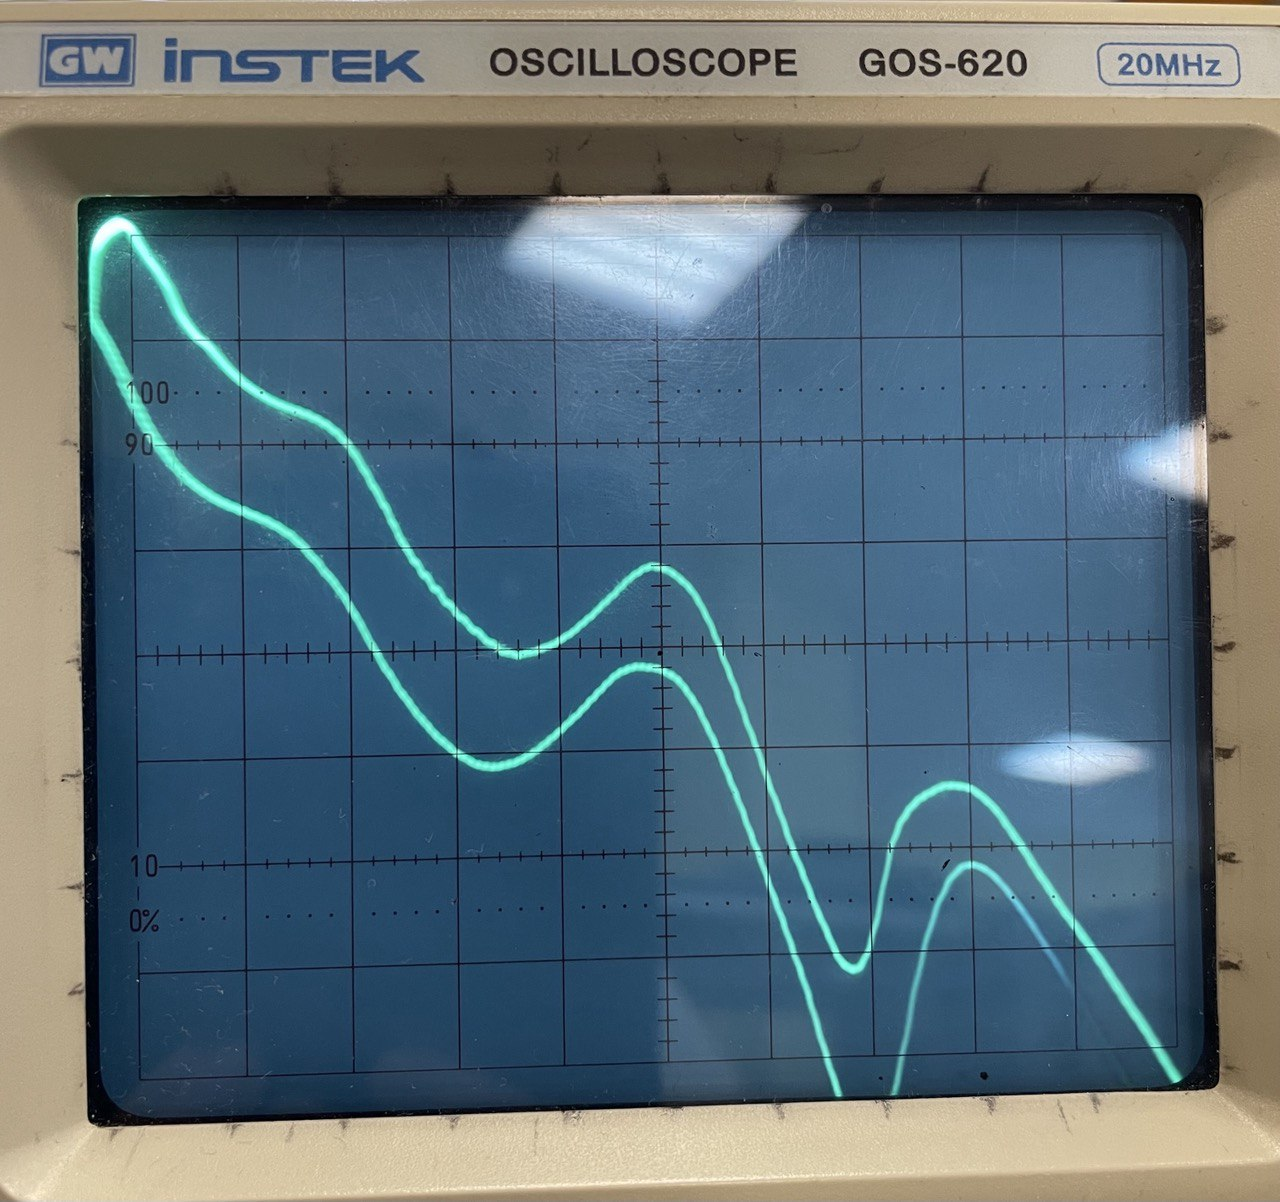
\includegraphics[width=9cm]{ex3.jpg}
    \caption{ВАХ на экране ЭО при V = 4B.}
    \label{fig:}
  \end{center}
\end{figure}

\item Получив средний результат $\Delta{V_{cr}}$ = 15.3 В, можем определить энергию возбуждения первого уровня атома гелия в электрон-вольтах

\[E_1 =  \Delta{V_{cr}} = 15.3 eB\]

\item Ошибка измерения учитывает приборную и среднестатистическую погрешности:

\[ \delta{V_{cr}} = \sqrt{\delta{V_{pr}}^2 + \delta{V_{ct}}^2} \]

 , где приборная $\delta{V_{pr}} = 0.5B$, а среднестатистическая $\delta{V_{ct}} = 0.4B$
 
 значит результат с учетом погрешности:
 
 \[E_1 = (15.3 \pm 0.6) eB\]
 

\item Также по начальному участку можно оценить значение котактной разности потенциалов, в нашем случае его значение составляет $\Delta{V_{con}}$ = 10 B.

    \begin{figure}[H]
  \begin{center}
    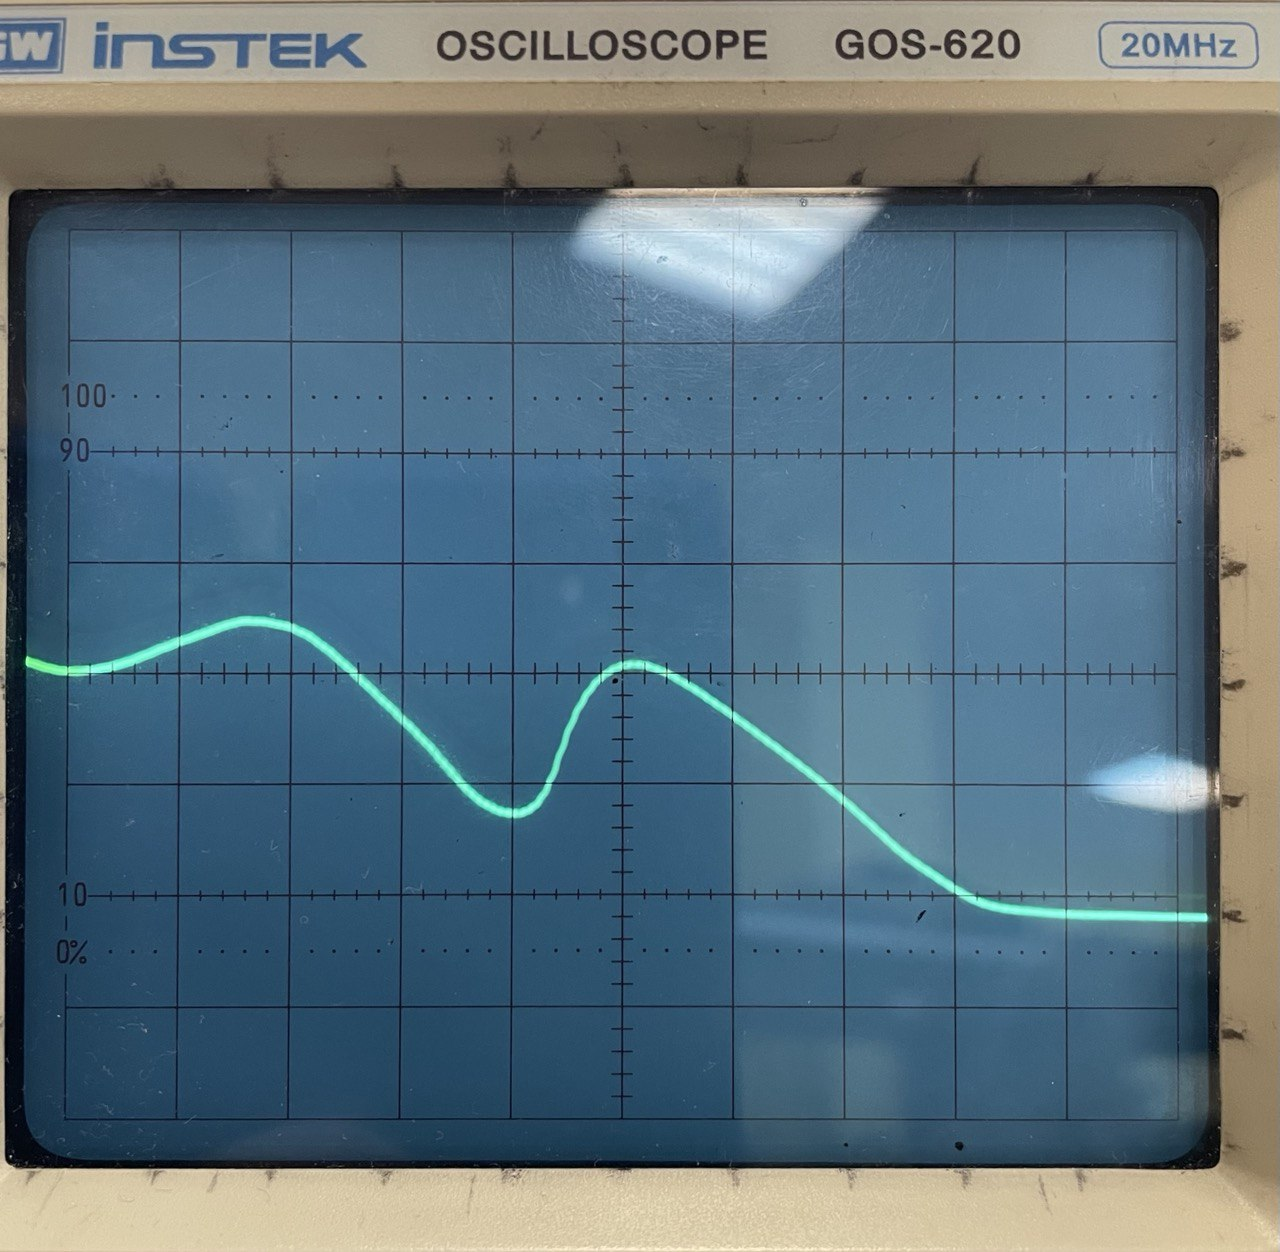
\includegraphics[width=9cm]{ex4.jpg}
    \caption{Контактная разность потенциалов.}
    \label{fig:}
  \end{center}
\end{figure}


 \end{enumerate}


\section{Статический режим} 
  
 
 \begin{enumerate}
\item При максимальном накале снимаем зависимость коллекторного тока от анодного напряжения ($I_k = f(V_a)$) для трех значений задерживающего напряжения V.

\item Строим графики зависимости для всех значений задерживающего напряжения V.

1.\textbf{V = 4B}

  \begin{table}[H]
\begin{center}
\begin{tabular}{|c|c|c|c|c|c|c|c|c|c|c|}
\hline $I_k , mkA $&9&71&145&205&225&232&199&180&198&235\\
\hline $V_a , B$&0.0&5.5&10.7&15.9&17.8&21.1&23.0&23.8&25.2&27.7\\
\hline $I_k , mkA $&271&330&360&347&338&354&380&410&500&510\\
\hline $V_a , B$&30.1&33.7&38.2&40.1&44.5&47.5&51.3&54.7&73.3&75.7\\
\hline
\end{tabular}
\end{center}
\end{table}


2.\textbf{V = 6B}

  \begin{table}[H]
\begin{center}
\begin{tabular}{|c|c|c|c|c|c|c|c|c|c|c|}
\hline $I_k , mkA $&1&76&152&198&228&212&129&182&237&305\\
\hline $V_a , B$&0.0&7.2&12.3&16.0&19.5&23.0&24.8&28.3&31.5&36.3\\
\hline $I_k , mkA $&310&274&277&286&312&312&362&382&395&390\\
\hline $V_a , B$&38.7&44.9&47.9&49.9&53.7&53.7&61.4&71.9&74.7&75.2\\
\hline
\end{tabular}
\end{center}
\end{table}


3.\textbf{V = 8B}


  \begin{table}[H]
\begin{center}
\begin{tabular}{|c|c|c|c|c|c|c|c|c|c|c|}
\hline $I_k , mkA $&4&61&146&191&217&186&107&87&141&197\\
\hline $V_a , B$&3.3&7.9&13.6&17.2&20.8&23.8&24.3&66.5&29.7&32.7\\
\hline $I_k , mkA $&243&255&242&216&209&236&267&280&283&291\\
\hline $V_a , B$&35.7&37.7&41.3&45.5&47.8&54.3&58.9&62.9&66.5&75.0\\
\hline
\end{tabular}
\end{center}
\end{table}

       \begin{figure}[H]
  \begin{center}
    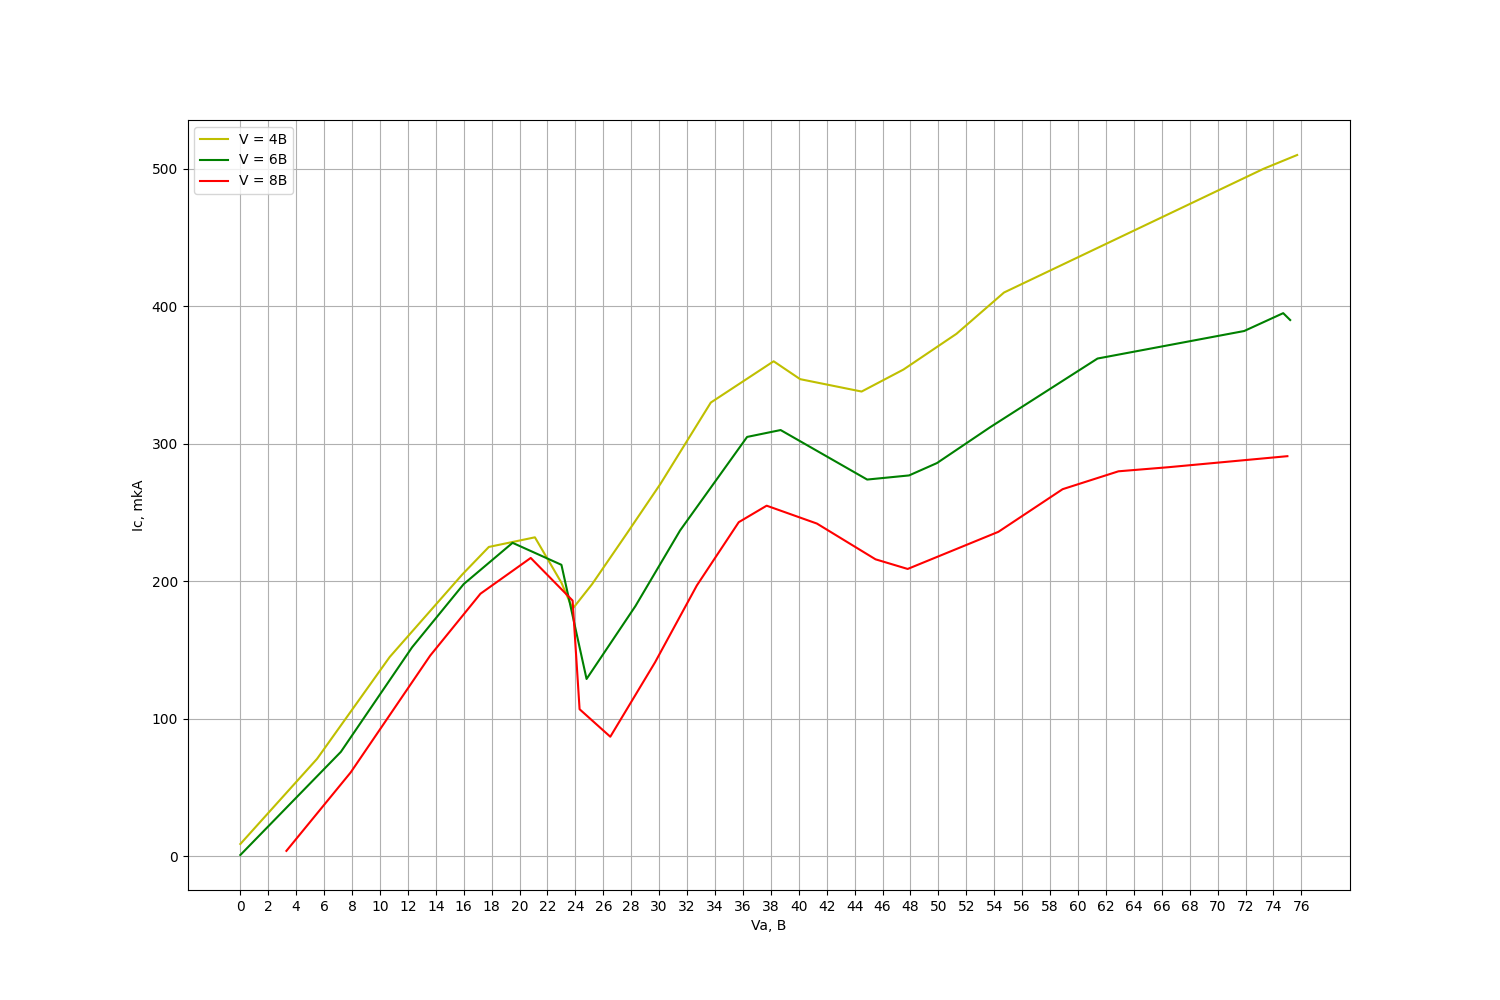
\includegraphics[width=20cm]{gra1.png}
    \caption{Статический режим.}
    \label{fig:}
  \end{center}
\end{figure}


\item По графикам заполняем таблицу, аналогичную динамическому режиму:

  \begin{table}[H]
\begin{center}
\begin{tabular}{|c|c|c|c|}
\hline $V $, B&$\Delta{V_1}$, дел &$\Delta{V_2}$, дел& $\Delta{V_{cr}}$, дел\\
\hline 4&22&20&21.0\\
\hline 6&23&20&21.5\\
\hline 8&22&22&22.0\\
\hline 
\end{tabular}
\end{center}
\end{table}

\item По данным таблицы определяем энергию возбуждения первого уровня атома гелия:

\[E_1 = \Delta{V_{cr}} = 21.5 eB\]

\item Ошибка измерения учитывает приборную, среднестатистическую и графическую погрешности:

\[ \delta{V_{cr}} = \sqrt{\delta{V_{pr}}^2 + \delta{V_{ct}}^2 + \delta{V_{gr}}^2} \]

 , где приборная $\delta{V_{pr}} = 0.05B$, среднестатистическая $\delta{V_{ct}} = 0.3B$, графическая $\delta{V_{gr}} = $0.5B
 
 значит результат с учетом погрешности:
 
 \[E_1 = (21.5 \pm 0.6) eB\]
 

\end{enumerate}


\section{Выводы}

В данной работе мы получили значения энергии возбуждения первого уровня атома гелия в:

$\newline$
1.) Динамическом режиме. Значение этой величины cocтавило  $E_1 = (15.3 \pm 0.6) eB$, что отличается от табличного значения $E = 21.6$ эВ на 29 \%.

2.) Статическом режиме. Значение этой величины составило $E_1 = (21.5 \pm 0.6) eB$, что отличается от табличного значения всего лишь на 0.5\% и совпадает с учетом погрешности.

Полученные результаты говорят о том, что измерения первого уровня возбуждения атома гелия в динамическом режиме дают гораздо большее отклонения от табличного значения, чем в статическом. Это связано с грубыми измерениями напряжения по электронному осциллографу и неточностью его показаний. Хорошие результаты в статическом режиме обусловлены точечным измерением ВАХ и чувствительностью приборов.


\end{document}
	
